% Relatório Técnico — Prática MLP
% Tópicos Avançados em Inteligência Artificial — UFRPE
% Template: Springer LNCS
\documentclass[runningheads]{llncs}

\usepackage[T1]{fontenc}
\usepackage[utf8]{inputenc}
\usepackage[portuguese]{babel}
\usepackage{graphicx}
\usepackage{booktabs}
\usepackage{amsmath}
\usepackage{hyperref}
\usepackage{float}

\begin{document}

\title{MLP do Zero: Classificação de Doença Cardíaca com Rede Neural
Implementada como Grafo}

\author{Rayane Thaís Gomes de Lima France\inst{1}}

\authorrunning{R. France}

\institute{Universidade Federal Rural de Pernambuco (UFRPE), Recife, PE, Brasil\\
\email{rayane.france@ufrpe.br}}

\maketitle

\begin{abstract}
Este relatório descreve a implementação de uma rede neural do tipo
Multi-Layer Perceptron (MLP) construída inteiramente do zero em Python,
representada internamente como um grafo explícito de nós e arestas.
A rede foi aplicada ao dataset UCI Heart Disease para classificação
binária de presença de doença cardíaca, atingindo 81,4\% de acurácia
no conjunto de teste após deduplicação de amostras. São apresentados
os resultados de seis variações experimentais de arquitetura,
taxa de aprendizagem e número de épocas.

\keywords{MLP \and Backpropagation \and Grafo \and Heart Disease \and
Classificação Binária}
\end{abstract}

% =====================================================================
\section{Introdução}
% =====================================================================

A atividade prática da disciplina de Tópicos Avançados em Inteligência
Artificial teve como objetivo a implementação manual de uma rede neural
MLP (Multi-Layer Perceptron) a partir da estrutura de um grafo, sem
utilizar frameworks como TensorFlow ou PyTorch.

As especificações foram:
\begin{enumerate}
    \item Codificar uma MLP a partir da estrutura de um grafo, com
          neurônios como nós e pesos como arestas;
    \item Implementar manualmente as funções de \textit{feed forward}
          e \textit{back propagation};
    \item Utilizar o dataset Heart Disease com divisão 80\% treino
          e 20\% teste;
    \item Demonstrar visualmente o progresso do treinamento e da
          inferência em tempo real.
\end{enumerate}

O dataset Heart Disease~\cite{ref_heart} contém registros de pacientes
com 13 atributos clínicos (idade, sexo, tipo de dor no peito,
pressão arterial, colesterol, entre outros) e um alvo binário indicando
presença ou ausência de doença cardíaca.

% =====================================================================
\section{Método}
% =====================================================================

\subsection{Organização do Projeto}

O projeto foi organizado seguindo o \textit{harness} acadêmico do
professor~\cite{ref_harness}, com a estrutura de pastas mostrada
na Figura~\ref{fig:arch}. O versionamento segue GitFlow, com
desenvolvimento na branch \texttt{feature/mlp-pratica-streamlit}
antes de ser integrado a \texttt{develop} e \texttt{main}.

\begin{figure}[H]
\centering
\small
\begin{verbatim}
ai4good/
├── code/
│   ├── src/mlp/
│   │   ├── graph.py       (MLPGraph, Neuron, Connection, Layer)
│   │   ├── data.py        (load, deduplicate, split, standardize)
│   │   ├── activations.py (relu, sigmoid + derivadas)
│   │   └── losses.py      (binary cross-entropy + derivada)
│   ├── scripts/
│   │   ├── mlp_streamlit.py  (interface visual)
│   │   └── run_experiments.py (variações de hiperparâmetros)
│   └── tests/             (16 testes automatizados)
├── article/               (este relatório — Overleaf)
└── tools/                 (workspace_check.py)
\end{verbatim}
\caption{Arquitetura de módulos do projeto. Setas de dependência:
\texttt{data.py} $\rightarrow$ \texttt{graph.py} $\rightarrow$
\texttt{mlp\_streamlit.py}.}
\label{fig:arch}
\end{figure}

\subsection{Bibliotecas e Ferramentas}

\begin{itemize}
    \item \textbf{NumPy} — operações matriciais para forward e backward
          acelerados;
    \item \textbf{Streamlit} — interface web interativa para
          treinamento e inferência em tempo real;
    \item \textbf{Matplotlib} — renderização do grafo da rede com
          camadas alinhadas;
    \item \textbf{Antigravity (Google)} — assistente de IA para
          codificação e organização do projeto;
    \item \textbf{Git + GitFlow} — versionamento com branches
          \texttt{feature/*} $\to$ \texttt{develop} $\to$ \texttt{main}.
\end{itemize}

\subsection{Representação como Grafo}

A MLP é representada internamente por três \textit{dataclasses}:

\begin{itemize}
    \item \textbf{Neuron} — nó do grafo com identificador, bias,
          pré-ativação ($z$), ativação ($a$) e delta ($\delta$);
    \item \textbf{Connection} — aresta com identificadores de origem
          e destino e peso numérico;
    \item \textbf{Layer} — grupo de neurônios com tipo de ativação
          (input, relu, sigmoid).
\end{itemize}

A classe \texttt{MLPGraph} orquestra a rede completa. Os pesos são
inicializados com Xavier/Glorot uniforme:
\[
w \sim U\left(-\sqrt{\frac{6}{n_{in}+n_{out}}},\;
+\sqrt{\frac{6}{n_{in}+n_{out}}}\right)
\]

\subsection{Feed Forward}

O forward pass percorre cada camada sequencialmente:
\[
z_j = \sum_i w_{ij} \cdot a_i + b_j, \qquad
a_j = \sigma(z_j)
\]
onde $\sigma$ é ReLU para camadas ocultas e Sigmoid para a saída.

\subsection{Backpropagation}

O gradiente da camada de saída, combinando BCE com Sigmoid, simplifica
para:
\[
\delta_{\text{saída}} = \hat{y} - y
\]

Para camadas ocultas, o delta é propagado pela regra da cadeia:
\[
\delta_j = \left(\sum_k w_{jk} \cdot \delta_k\right) \cdot
\sigma'(z_j)
\]

A atualização dos pesos segue SGD puro:
\[
w_{ij} \leftarrow w_{ij} - \eta \cdot \delta_j \cdot a_i, \qquad
b_j \leftarrow b_j - \eta \cdot \delta_j
\]

A corretude do backward foi verificada por \textit{gradient checking}
numérico com diferenças centrais ($\epsilon = 10^{-5}$, tolerância
$< 10^{-4}$), implementado em 4 testes automatizados.

\subsection{Pré-processamento}

O dataset Kaggle \texttt{johnsmith88/heart-disease-dataset} possui
1.025 registros, mas apenas \textbf{302 são únicos} — 723 linhas
são duplicatas com labels consistentes. Sem deduplicação, amostras
idênticas caem em treino e teste, inflando artificialmente a acurácia
para 100\%.

Etapas aplicadas:
\begin{enumerate}
    \item \textbf{Deduplicação} — remoção de linhas repetidas
          (\texttt{np.unique} com \texttt{return\_index});
    \item \textbf{Divisão estratificada} — 80/20 por classe,
          sem sobreposição, semente 42;
    \item \textbf{Padronização Z-score} — média e desvio-padrão
          calculados \textit{exclusivamente} no treino e aplicados
          ao teste.
\end{enumerate}

% =====================================================================
\section{Resultados e Discussão}
% =====================================================================

\subsection{Visualização da Rede}

A Figura~\ref{fig:before_after} mostra a arquitetura da rede
(13\,|\,8\,|\,5\,|\,1) visualizada em dois momentos: antes do
treinamento (pesos iniciais Xavier) e após 60 épocas de SGD.
As arestas azuis representam pesos positivos e as vermelhas,
pesos negativos; a espessura é proporcional à magnitude.

Após o treinamento, observa-se uma clara diferenciação: algumas
conexões se fortalecem enquanto outras se enfraquecem, indicando
que a rede aprendeu a distinguir padrões relevantes para a
classificação.

\begin{figure}[H]
\centering
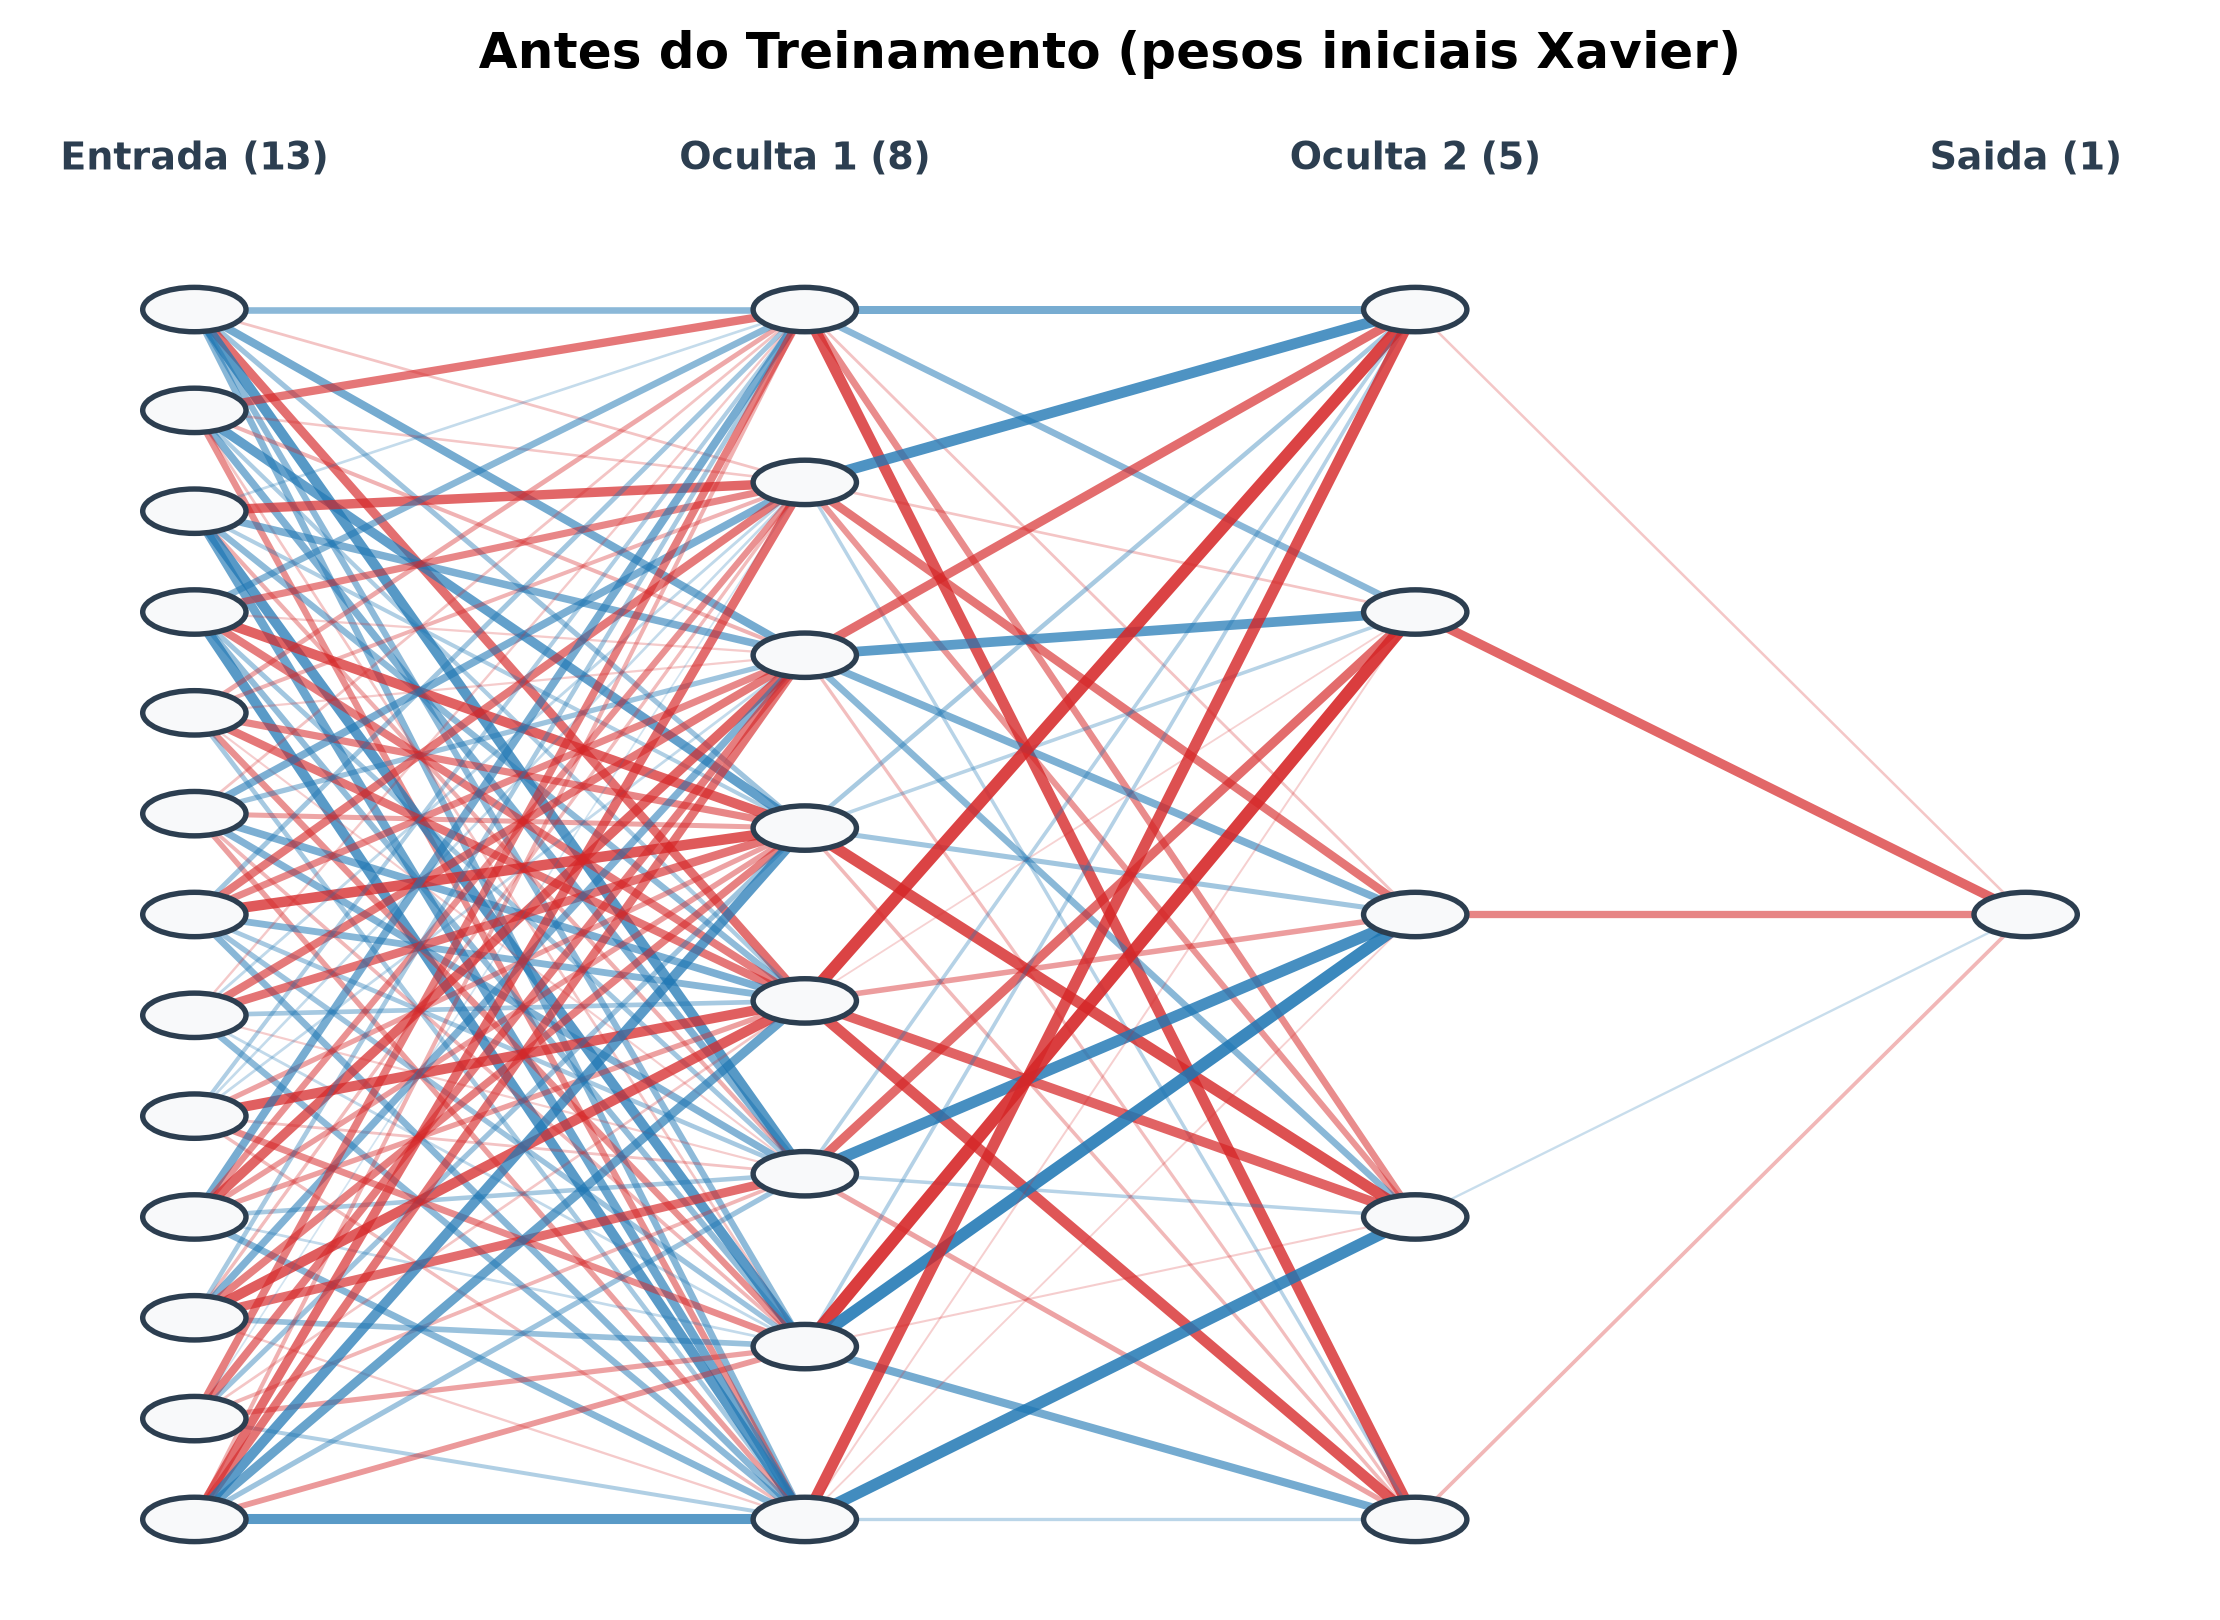
\includegraphics[width=0.48\textwidth]{mlp_graph_before.png}
\hfill
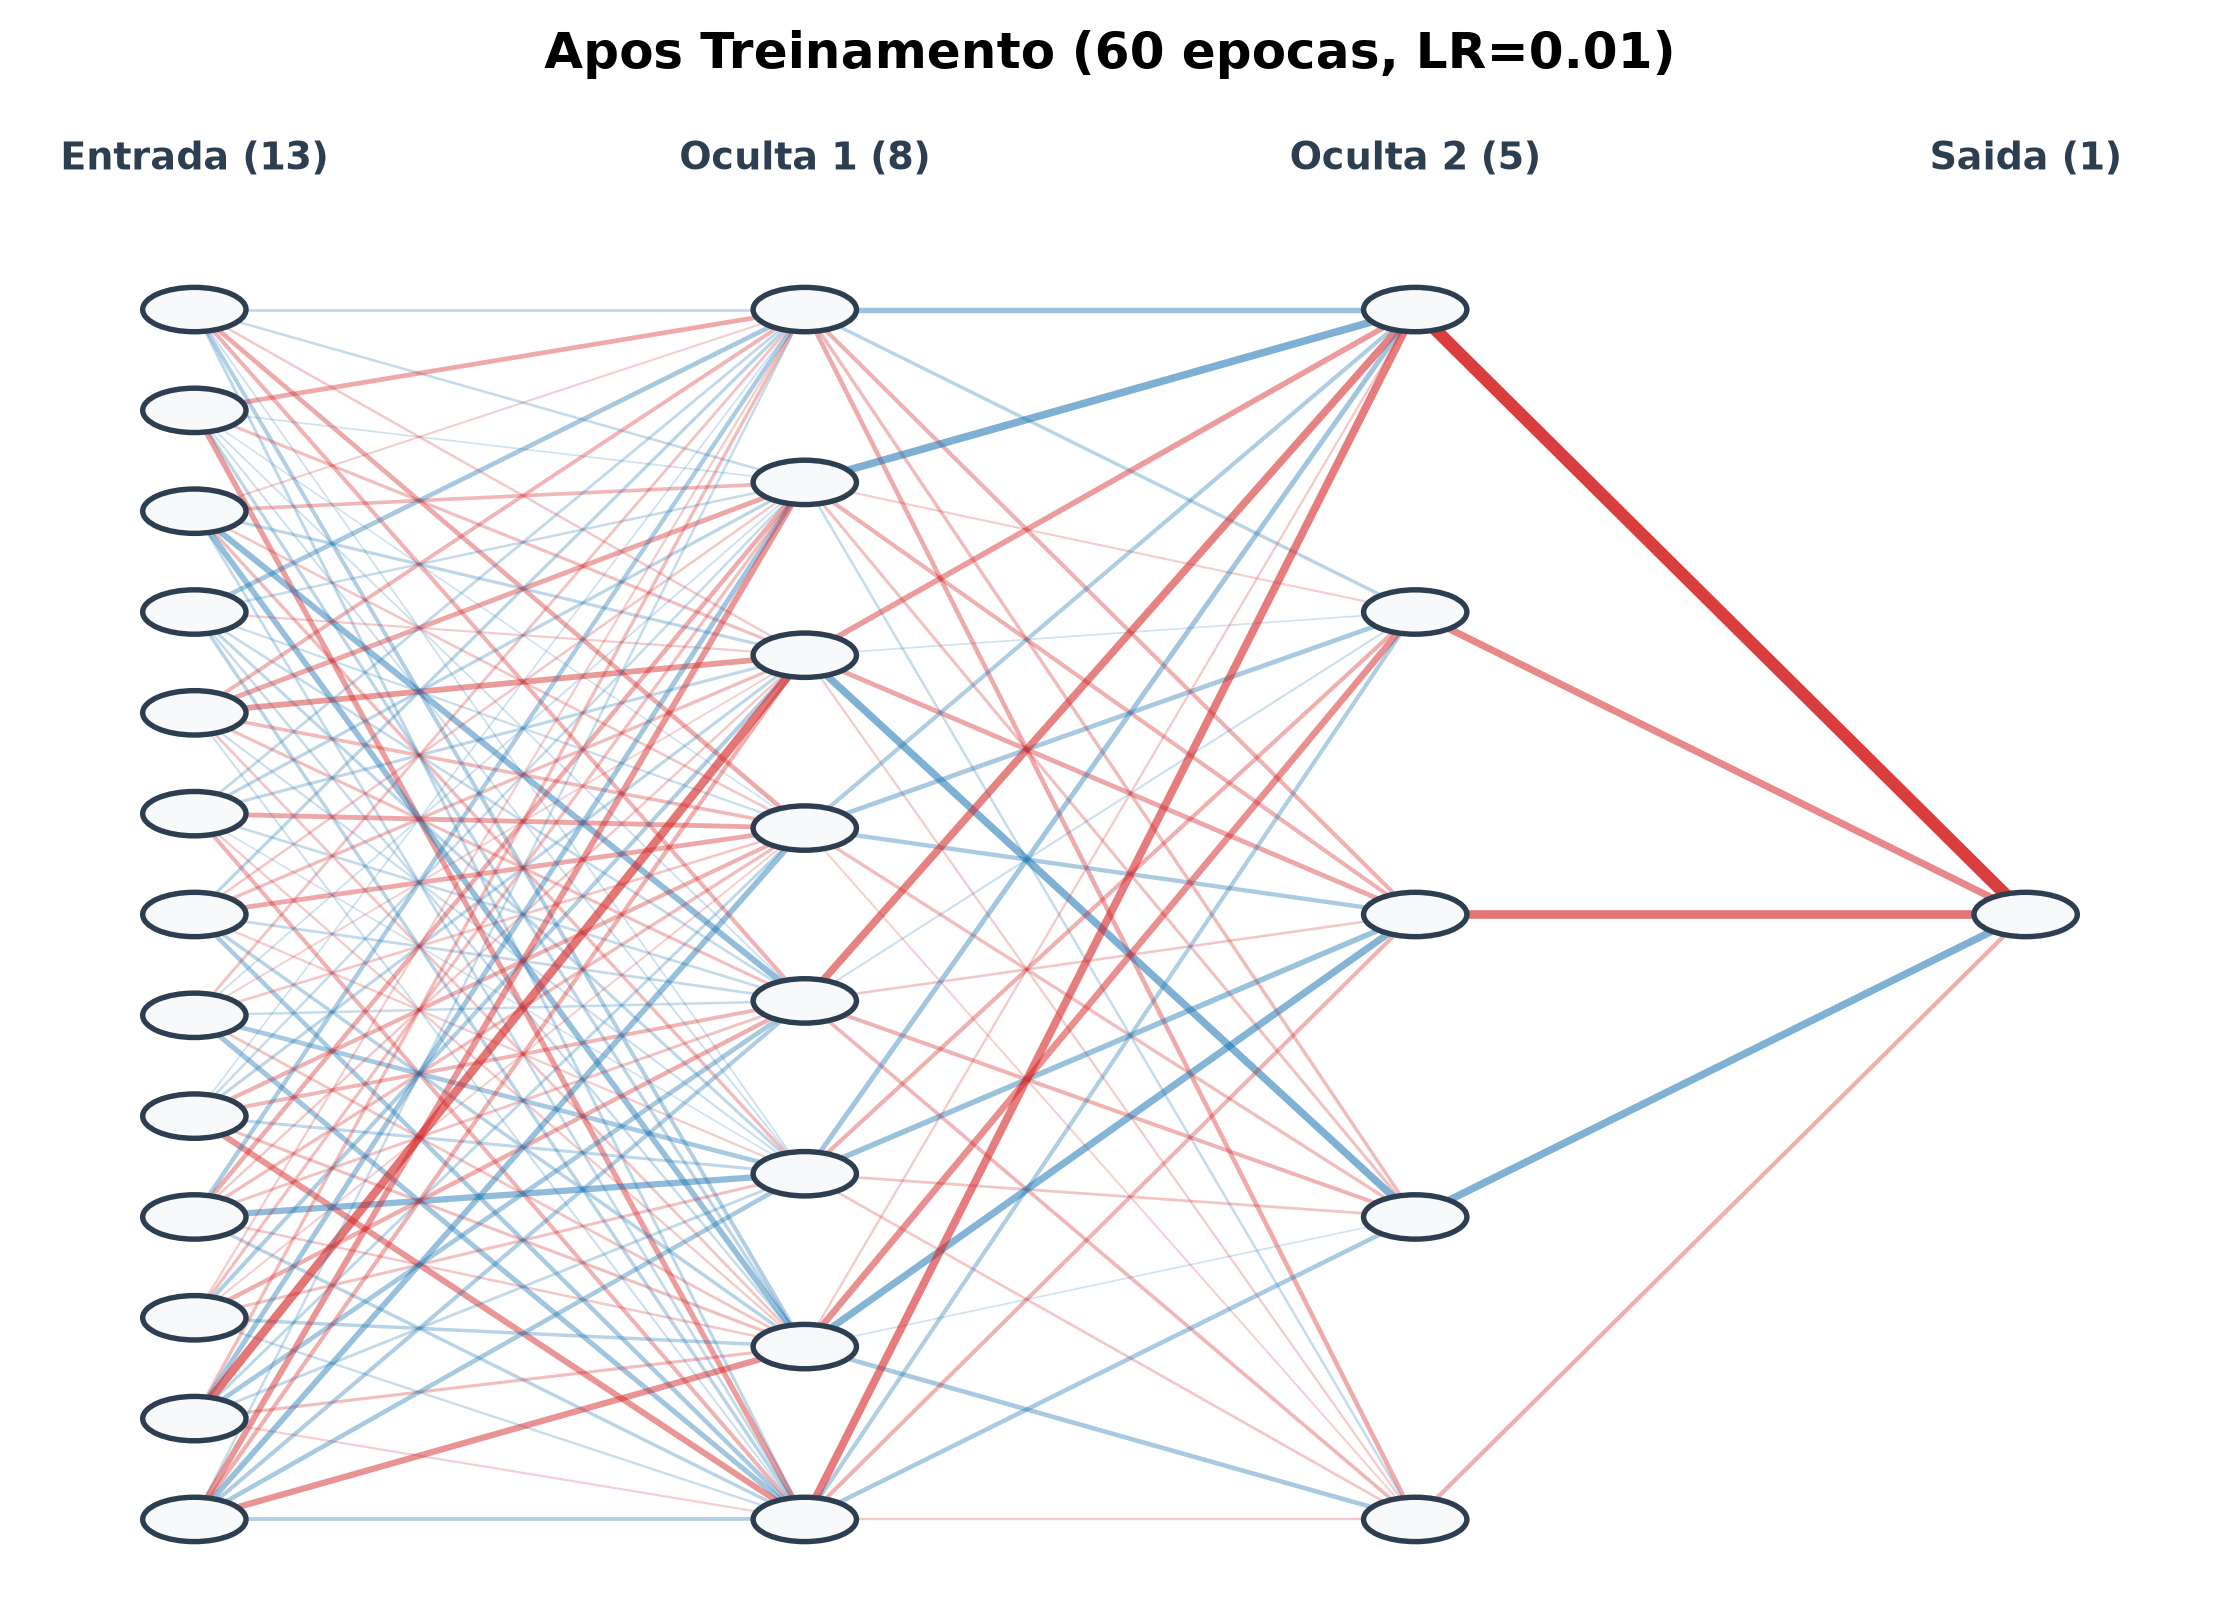
\includegraphics[width=0.48\textwidth]{mlp_graph_after.png}
\caption{Grafo da MLP antes (pesos iniciais Xavier) e depois do treinamento
(60 épocas, $\text{LR}=0{,}01$). Arestas azuis indicam pesos positivos e
vermelhas, pesos negativos; a espessura é proporcional à magnitude.}
\label{fig:before_after}
\end{figure}

\subsection{Métricas do Modelo Baseline}

A configuração baseline (13\,|\,8\,|\,5\,|\,1, $\text{LR}=0{,}01$, 60 épocas)
obteve os resultados apresentados na Tabela~\ref{tab:baseline}.

\begin{table}[H]
\centering
\caption{Métricas do modelo baseline no conjunto de teste (59 amostras).}
\label{tab:baseline}
\begin{tabular}{@{}lc@{}}
\toprule
\textbf{Métrica} & \textbf{Valor} \\
\midrule
Acurácia (teste) & 0,8136 (81,4\%) \\
Acurácia (treino) & 0,9712 (97,1\%) \\
Loss final (treino) & 0,1299 \\
Precision (classe 1) & 0,8182 \\
Recall (classe 1) & 0,8438 \\
F1-Score (classe 1) & 0,8308 \\
Total de conexões & 149 \\
Tempo de treinamento & 2,79 s \\
\bottomrule
\end{tabular}
\end{table}

\subsection{Variações Experimentais}

Para investigar o comportamento da MLP sob diferentes hiperparâmetros,
foram avaliadas seis configurações, resumidas na Tabela~\ref{tab:experiments}.

\begin{table}[H]
\centering
\caption{Comparação de variações de arquitetura, taxa de aprendizagem e épocas.}
\label{tab:experiments}
\begin{tabular}{@{}lcccccc@{}}
\toprule
\textbf{Experimento} & \textbf{Arquitetura} & \textbf{LR} &
\textbf{Ép.} & \textbf{Acc Test} & \textbf{Acc Train} &
\textbf{F1} \\
\midrule
Baseline         & 13\,|\,8\,|\,5\,|\,1   & 0,01  & 60  & 0,8136 & 0,9712 & 0,8308 \\
Rede menor       & 13\,|\,4\,|\,1         & 0,01  & 60  & \textbf{0,8644} & 0,8930 & \textbf{0,8824} \\
Rede maior       & 13\,|\,16\,|\,8\,|\,1  & 0,01  & 60  & 0,8305 & 0,9918 & 0,8485 \\
LR alta          & 13\,|\,8\,|\,5\,|\,1   & 0,05  & 60  & 0,7966 & 0,9053 & 0,8065 \\
LR baixa         & 13\,|\,8\,|\,5\,|\,1   & 0,001 & 60  & 0,8305 & 0,8436 & 0,8438 \\
200 épocas       & 13\,|\,8\,|\,5\,|\,1   & 0,01  & 200 & 0,8305 & 1,0000 & 0,8387 \\
\bottomrule
\end{tabular}
\end{table}

\paragraph{Impacto da arquitetura.}
Notavelmente, a \textbf{rede menor} (13\,|\,4\,|\,1, apenas 61 conexões)
obteve o melhor resultado de teste ($86{,}44\%$ de acurácia e F1 de $0{,}8824$),
superando o baseline e a rede maior. Esse comportamento exemplifica o princípio
da parcimônia (Navalha de Ockham): como o conjunto de treino conta com apenas
243 instâncias únicas, uma capacidade representacional mais restrita atua como
um regularizador intrínseco, prevenindo a memorização de ruído amostral.
Por outro lado, a rede maior (13\,|\,16\,|\,8\,|\,1, 361 conexões) alcançou
$99{,}18\%$ no treino e $83{,}05\%$ no teste, evidenciando o início de
sobreajuste (\textit{overfitting}).

\paragraph{Impacto da taxa de aprendizagem.}
Com $\text{LR}=0{,}05$, observou-se instabilidade na convergência: os passos
no espaço de parâmetros foram excessivamente grandes, resultando na menor
acurácia de teste ($79{,}66\%$) e maior perda residual ($0{,}2393$).
Com $\text{LR}=0{,}001$, a rede aprendeu de maneira estável, porém lenta,
atingindo acurácia de teste de $83{,}05\%$ com loss de treino ainda em
$0{,}4286$ ao fim das 60 épocas. A taxa $\text{LR}=0{,}01$ provou ser
o ponto ótimo de equilíbrio entre velocidade de convergência e estabilidade.

\paragraph{Impacto do número de épocas e sobreajuste.}
Ao elevar o treinamento para 200 épocas, a rede atingiu $100\%$ de acurácia no
conjunto de treinamento com perda praticamente nula ($0{,}0084$). Contudo,
a acurácia de teste não acompanhou esse ganho, permanecendo em $83{,}05\%$.
Essa disparidade ($100\%$ vs.\ $83{,}1\%$) demonstra empiricamente a
memorização do conjunto de treinamento, reforçando a importância prática de
mecanismos de parada antecipada (\textit{early stopping}) ou técnicas de
regularização (\textit{dropout}, penalização $L_2$).

\section{Conclusão}

A implementação manual da MLP em estrutura de grafo permitiu compreender
em detalhe o fluxo de tensores e derivadas parciais que regem o aprendizado
profundo. A deduplicação dos dados foi um passo metodológico crucial para
garantir uma avaliação honesta de generalização, evitando a acurácia espúria
de 100\%. Os experimentos demonstraram que, para bases médicas tabulares de
pequeno porte como o Heart Disease, redes compactas com regularização natural
frequentemente superam arquiteturas mais profundas.

% =====================================================================
% Referências
% =====================================================================

\begin{thebibliography}{3}

\bibitem{ref_heart}
Lapp, D.: Heart Disease Dataset.
Kaggle, \url{https://www.kaggle.com/datasets/johnsmith88/heart-disease-dataset} (2017).
Baseado em: Janosi, A., Steinbrunn, W., Pfisterer, M., Detrano, R.:
UCI Heart Disease. \url{https://archive.ics.uci.edu/dataset/45/heart+disease}

\bibitem{ref_harness}
Figueiredo, L.S.: AI4Good Workspace.
GitHub, \url{https://github.com/lsfcin/workspace} (2024)

\bibitem{ref_glorot}
Glorot, X., Bengio, Y.: Understanding the difficulty of training
deep feedforward neural networks. In: Proceedings of the 13th
International Conference on Artificial Intelligence and Statistics
(AISTATS), pp. 249--256 (2010)

\end{thebibliography}

\end{document}
